\documentclass[journal,10pt,twocolumn]{article}
\usepackage[margin=0.5in]{geometry}
\usepackage[cmex10]{amsmath}
\usepackage{amsmath}
\usepackage{array}
\usepackage{booktabs}
% The preceding line is only needed to identify funding in the first footnote. If that is unneeded, please comment it out.
\usepackage{cite}
\usepackage{amsmath,amssymb,amsfonts}
\usepackage{graphicx}
\usepackage{textcomp}
\usepackage{xcolor}
\usepackage{graphicx}
\graphicspath{{./fig}}{}
\def\BibTeX{{\rm B\kern-.05em{\sc i\kern-.025em b}\kern-.08em
    T\kern-.1667em\lower.7ex\hbox{E}\kern-.125emX}}
\usepackage{tikz}
\usetikzlibrary{shapes.geometric}
\usetikzlibrary{shapes.geometric,angles,quotes}
\usepackage{mathtools}  
\usepackage{diffcoeff}  

\begin{document}
\newtheorem{theorem}{Theorem}[section]
\newtheorem{problem}{Problem}
\newtheorem{proposition}{Proposition}[section]
\newtheorem{lemma}{Lemma}[section]
\newtheorem{corollary}[theorem]{Corollary}
\newtheorem{example}{Example}[section]
\newtheorem{definition}[problem]{Definition}
%\newtheorem{thm}{Theorem}[section] 
%\newtheorem{defn}[thm]{Definition}
%\newtheorem{algorithm}{Algorithm}[section]
%\newtheorem{cor}{Corollary}
\newcommand{\BEQA}{\begin{eqnarray}}
\newcommand{\EEQA}{\end{eqnarray}}
\newcommand{\define}{\stackrel{\triangle}{=}}
\newcommand*\circled[1]{\tikz[baseline=(char.base)]{
    \node[shape=circle,draw,inner sep=2pt] (char) {#1};}}
\bibliographystyle{article}
%\bibliographystyle{ieeetr}
\providecommand{\mbf}{\mathbf}
\providecommand{\pr}[1]{\ensuremath{\Pr\left(#1\right)}}
\providecommand{\re}[1]{\ensuremath{\text{Re}\left(#1\right)}}
\providecommand{\im}[1]{\ensuremath{\text{Im}\left(#1\right)}}
\providecommand{\qfunc}[1]{\ensuremath{Q\left(#1\right)}}
\providecommand{\sbrak}[1]{\ensuremath{{}\left[#1\right]}}
\providecommand{\lsbrak}[1]{\ensuremath{{}\left[#1\right.}}
\providecommand{\rsbrak}[1]{\ensuremath{{}\left.#1\right]}}
\providecommand{\brak}[1]{\ensuremath{\left(#1\right)}}
\providecommand{\lbrak}[1]{\ensuremath{\left(#1\right.}}
\providecommand{\rbrak}[1]{\ensuremath{\left.#1\right)}}
\providecommand{\cbrak}[1]{\ensuremath{\left\{#1\right\}}}
\providecommand{\lcbrak}[1]{\ensuremath{\left\{#1\right.}}
\providecommand{\rcbrak}[1]{\ensuremath{\left.#1\right\}}}
\newcommand{\sgn}{\mathop{\mathrm{sgn}}}
%\providecommand{\hilbert}{\overset{\mathcal{H}}{ \rightleftharpoons}}
\providecommand{\system}{\overset{\mathcal{H}}{ \longleftrightarrow}}
	%\newcommand{\solution}[2]{\textbf{Solution:}{#1}}
\newcommand{\solution}{\noindent \textbf{Solution: }}
\newcommand{\cosec}{\,\text{cosec}\,}
\providecommand{\dec}[2]{\ensuremath{\overset{#1}{\underset{#2}{\gtrless}}}}
\newcommand{\myvec}[1]{\ensuremath{\begin{pmatrix}#1\end{pmatrix}}}
\newcommand{\mydet}[1]{\ensuremath{\begin{vmatrix}#1\end{vmatrix}}}
	\newcommand*{\permcomb}[4][0mu]{{{}^{#3}\mkern#1#2_{#4}}}
\newcommand*{\perm}[1][-3mu]{\permcomb[#1]{P}}
\newcommand*{\comb}[1][-1mu]{\permcomb[#1]{C}}
%\numberwithin{equation}{section}
\numberwithin{equation}{subsection}
%\numberwithin{problem}{section}
%\numberwithin{definition}{section}
\let\vec\mathbf
\title{
{Finding the maxima and minima of the function \\
Using Advanced Optimization}\\
\thanks {Meer Tabres Ali as an intern with FWC IIT Hyderabad. *The author is with the Department of Electrical Engineering, Indian Institute of Technology, Hyderabad 502285 India e-mail: gadepall@iith.ac.in. All content in this manual is released under GNU GPL. Free and open source.}
}
\author{Meer Tabres Ali and G V V Sharma}
\maketitle
\tableofcontents
\section{Problem statement}
\begin{flushleft}
Determine the points of maxima and minima of the function\\
\vspace{0.25cm}
$f(x)$=$\frac{1}{8}lnx-bx+x^2, x>0$, where $b\geq0$ is a constant.
\end{flushleft}

\section{Considerations}
\vspace{0.2cm}
\begin{flushleft}
As per given data, the following table has been prepared.\\
\end{flushleft}
\vspace{0.3cm}
\begin{table}[htbp]
    \centering
\setlength\extrarowheight{2pt}
\begin{tabular}{|c|c|c|} \hline
      \textbf{Symbol}           &   \textbf{Value}   & \textbf{Description}\\ \hline
	f(x) & $\frac{1}{8}lnx-bx+x^2$ & function\\  \hline
	b & 7 & b$\geq0$\\ \hline
	a & $\frac{1}{8}$ & Coeff. of lnx\\ \hline
    c & 1 & Coeff. of $x^2$ \\ \hline

\end{tabular}
\caption{\label{tab:widgets}Considerations}
\end{table}

\section{Plot to find maxima and minima of the function}
\vspace{0.25cm}
Plot of the function $\frac{1}{8}lnx-bx+x^2$ is shown in the figure 1.
\begin{figure}[h]
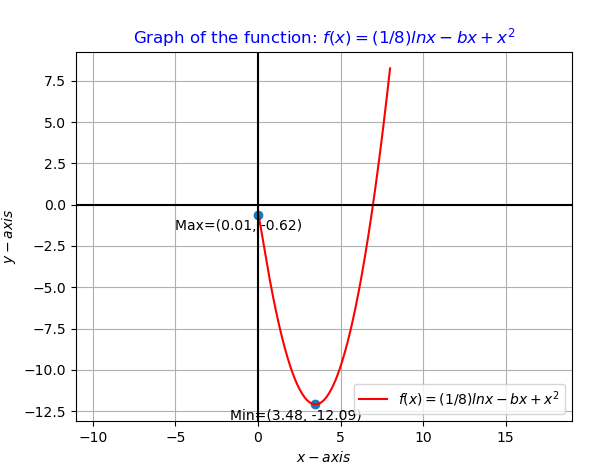
\includegraphics[width=1\columnwidth]{optadv.png}
\caption{Plot of f(x) to find Maxima and Minima}
\label{Optimization of Machince A and B}
\end{figure}

\section{Solution}
\begin{flushleft}
Given function is,\\
\end{flushleft}
\begin{equation}
    f(x)=\frac{1}{8}lnx-bx+x^2
\end{equation}
\begin{center}
where $x>0$ and $b\geq0$
\end{center}

\subsection{Calculation of Maxima and Minima using normal differentiation}
\begin{flushleft}
\vspace{0.35cm}
Differentiating above Eq. (4.0.1), we get,
\end{flushleft}
\vspace{0.25cm}
\center
$\diff{f(x)}{x}$ = $\diff{(\frac{1}{8}lnx-bx+x^2)}{x}$
\endcenter
\vspace{0.25cm}
\center
$\implies \diff{f(x)}{x}$ = $\frac{1}{8x}-b+2x$
\endcenter
\vspace{0.25cm}
\center
$\implies 0 = \frac{1}{8x}-b+2x$
\endcenter
\vspace{0.25cm}
\center
$\implies 16x^2-8bx+1=0$
\endcenter
\begin{flushleft}
On simplifying,
\end{flushleft}
\begin{equation}
  x_{max}=\frac{-b-\sqrt{b^2-1}}{4}, \hspace{0.2cm} x_{min}=\frac{-b+\sqrt{b^2-1}}{4}
\end{equation}
\begin{flushleft}
\vspace{0.15cm}
Assuming b=7,
\end{flushleft}
\begin{center}
  $x_{max}=0.01$
\end{center}
\begin{center}
\vspace{0.1cm}
 $x_{min}=3.48$
\end{center}
\begin{flushleft}
\vspace{0.1cm}
By submitting $x_{max}$ and $x_{min}$ in Eq. 4.0.1, we get,
\end{flushleft}
\vspace{0.2cm}
\begin{center}
 $f(x)_{max}=-0.62$
\end{center}
\begin{center}
$f(x)_{min}=-12.09$
\end{center}
\begin{flushleft}
Therefore,
\end{flushleft}
\begin{equation}
    Maximum \hspace{0.1cm}value \hspace{0.1cm}of \hspace{0.1cm} x \hspace{0.1cm}is \hspace{0.2cm}\textbf{-0.62} \hspace{0.2cm}at\hspace{0.2cm} x=\textbf{0.01}
\end{equation}
\begin{equation}
    Minimum \hspace{0.1cm}value \hspace{0.1cm}of \hspace{0.1cm}x \hspace{0.1cm}is\hspace{0.2cm} \textbf{-12.09} \hspace{0.2cm} at \hspace{0.2cm} x=\textbf{3.48}
\end{equation}

\begin{flushleft}
\subsection{Calculation of Maxima using gradient ascent algorithm}
\end{flushleft}

\begin{flushleft}
Maxima of the above equation (4.0.1), can be calculated from the following expression,\\
\end{flushleft}
\vspace{0.25cm}
    \begin{align}
        x_{n+1} &= x_n - \alpha \nabla f(x_n) \\
        \vspace{0.35cm}
        \implies x_{n+1} &= x_n - \alpha \brak{\frac{1}{8}(1/x_n)-7+2x_n}
    \end{align}
\begin{flushleft}
Taking $x_0=0.5,\alpha=0.001$ and precision = 0.00000001, values obtained using python are:
\end{flushleft} 
\vspace{0.35cm}
\center
        \boxed{$\text{Maxima} = -0.62$}\\
        \vspace{0.45cm}
        \boxed{$\text{Maxima Point} = 0.01$}
\endcenter
\begin{flushleft}
\subsection{Calculation of Minima using gradient descent algorithm}
\end{flushleft}
\begin{flushleft}
Maxima of the above equation (4.0.1), can be calculated from the following expression,\\
\end{flushleft}
\vspace{0.25cm}
    \begin{align}
        x_{n+1} &= x_n + \alpha \nabla f(x_n) \\
        \vspace{0.35cm}
        \implies x_{n+1} &= x_n + \alpha \brak{\frac{1}{8}(1/x_n)-7+2x_n}
    \end{align}
\begin{flushleft}
Taking $x_0=1.5,\alpha=0.001$ and precision = 0.00000001, values obtained using python are:
\end{flushleft} 
\vspace{0.35cm}
\center
        \boxed{$\text{Minima} = -12.09$}\\
        \vspace{0.45cm}
        \boxed{$\text{Minima Point} = 3.48$}
\endcenter
\section{Software}
\begin{flushleft}
Download the codes given in the link below and execute them.\\
\end{flushleft}

\begin{table}[h]
\centering
\begin{tabular}{|c|} \hline
\rule{0pt}{10pt} 
https://github.com/meertabresali-FWC-IITH/project/blob \\
/main/Asgn8.opt.advance/codes/optadv.py\\
\\\hline
 \end{tabular}
\end{table}




\section{Conclusion}
\begin{flushleft}
1. At first, the given function has been differentiated and it is solved by setting f'(x) equal to zero. By using x values, f(x) values are calculated.\\
\vspace{0.25cm}
2. Later, the given function f(x) is solved by gradient ascent algorithm to find maxima and the point at which f(x) is maximum.\\
\vspace{0.25cm}
3. Then, the given function f(x) is solved by gradient descent algorithm to find minima and the point at which f(x) is is minimum.\\
\vspace{0.25cm}
4. Maxima and Minima and related points are, \\
\vspace{0.25cm}
\center
Maxima point, Max=(0.01, -0.62) and\\ 
\vspace{0.2cm}
Minima point, Min=(3.48, -12.09)
\end{flushleft}
\endcenter
\end{document}
